
\section{Einleitung}
In diesem Versuch wird das Scanverfahren in der Ultraschalltechnik angewendet.
\newline
Zu erst werden die Fehlstellen eines Acrylblocks mit dem Scanverfahren bestimmt.
Danach wird an einem Herzmodell die Herzfrequenz und das Herzvolumen aufgenommen.
\section{Theorie}
Dem Ultraschall wird ein Frequenzbereich von ungefähr 20\,Hz bis 1\,GHz zugeordnet.
Der Schall ist allgemein eine longitudinale Welle, die aufgrund von Druckschwankungen
weitergeleitet wird. Diese lässt sich durch
\begin{equation}
  p(x,t) = p\ua{0} + v\ua{0}Z\cos{\omega t - kx}
  \label{eqn:Welle}
\end{equation}
beschreiben. Die akustische Impedanz Z ist abhängig von der Dichte $\rho$ des zu untersuchenden
Materials und der Schallgeschwindigkeit c. Der Zusammenhang lautet wie folgt
\begin{equation}
  Z = c \cdot \rho.
\end{equation}
In Gasen und Flüssigkeiten breiten sich die Schallwellen nur longitudinal aus
\begin{equation}
  c\ua{Fl} = \sqrt{ \frac{1}{\kappa \cdot \rho} }.
\end{equation}
$\kappa$ ist dabei das Kompressibilitätsmodul.
\newline
Bei Festkörpern kommt es neben der longitudinalen Schallwellenausbreitung auch
noch zu einer transversalen Ausbreitung des Ultraschalls. Mit dem Elastizitätsmodul E ergibt sich
dann der folgende Zusammenhang für die Schallgeschwindigkeit
\begin{equation}
  c\ua{Fe} = \sqrt{ \frac{E}{\rho}}.
\end{equation}
Beim Übergang von den Ultraschallwellen in ein anderes Medium kommt es aufgrund der Transmission
zur Absorption von Energie. Die Intensität des Ultraschall nimmt exponentiell mit der
Strecke ab
\begin{equation}
  I(\su{x}) = I\ua{0} \cdot e^{-\alpha \su{x}}.
\end{equation}
Dabei ist $\su{I_0}$ die Anfangsintenstität, $\alpha$ der Absorptionskoeffizient und x die zurückgelegte Strecke.
Der Absorptionskoeffizient von Luft ist sehr groß, weshalb ein Kontaktmittel wie bidestilliertes
Wasser verwendet wird, um diesen gering zu halten.
\newline
Das Verhältnis der einfallenden zur reflektieren Intensität wird über den Reflektionskoeffizienten
beschrieben. Dieser ist abhängig von den Impedanzen beider Medien an der Grenzfläche
\begin{equation}
  R = \left( \frac{Z\ua{1} - Z\ua{2}}{Z\ua{1} + Z\ua{2}} \right)^2.
\end{equation}
Für den Transmissionskoeffizienten gilt T = 1\,$-$\,R.

Die Erzeugung des Ultraschalls ergibt sich durch den reziproken piezo-elektrischen Effekt.
In einem elektrischen Wechselfeld wird ein Piezokristall zu Schwingungen und somit zur
Aussendung von Ultraschallwellen angeregt. Für besonders hohe Intensitäten kommt es
zur Resonanz. Hierbei ist die Anregungs- gleich der Eigenfrequenz des Kristalls.
Piezokristalle können nicht nur als Sender verwendet werden, sondern auch als Empfänger
beim Impuls-Echo-Verfahren.
\newline
In der Ultraschalltechnik kommt es zur Anwendung zweier Verfahren.
\newline
Das erste ist das Durschallungsverfahren. Die zu untersuchende Probe wird zwischen Ultraschallsender und
-empfänger plaziert. Durch Aussendung eines kurzzeitigen Schallimpulses kann die empfangene
Intensität Rückschluss auf vorhandene Fehlstellen liefern.
\newline
Die zweite Vorgehensweise ist das Impuls-Echo-Verfahren. Hierbei fungiert der Ultraschallsender
auch als Empfänger. Nach der Reflektion des Ultraschall an einer Grenzflächen, kehrt dieser
zum Empfänger zurück. Die Höhe des Echos liefert eine Aussage über die Größe der Fehlstellen.
Bei einer bekannter Schallgeschwindigkeit c im zu untersuchenden Medium, kann über die Laufzeitmessung
die Lage der Fehlstelle festgestellt werden
\begin{equation}
  s = \frac{1}{2} c\,t.
\end{equation}
Die Laufzeit kann über drei verschiedenen Scans dargestellt werden.
Über den A-Scan (Amplitude-Scan) wird die Amplitude der registrierten Welle sichtbar gemacht.
Beim B-Scan (Brightness-Scan) wird die aufgenommene Echoamplitude in Helligkeitsabstufungen dargestellt.
Durch das Bewegen der Ultraschallsonde entseht so ein zweidimensionales Bild.
Beim TM-Scan (Time-Motion-Scan) können durch schnelles Abtasten Bewegungen sichtbar gemacht werden.
\section{Durchführung}
Vor Beginn der Ultraschallmessung werden die Abmessungen des Acrylblocks bestimmt.
Mit bidestillierten Wasser als Kontaktflüssigkeit werden von oben und von unten die
Strecken zu den jeweiligen Fehlstellen mit einer 1\,MHz Ultraschallsonde ausgemessen.
Außerdem werden die Durchmesser der einzelnen Fehlstellen aufgenommen.
\newline
In Abbildung \ref{fig:fehl} sind die Fehlstellen des Acrylblocks dargestellt.
\begin{figure}
  \centering
  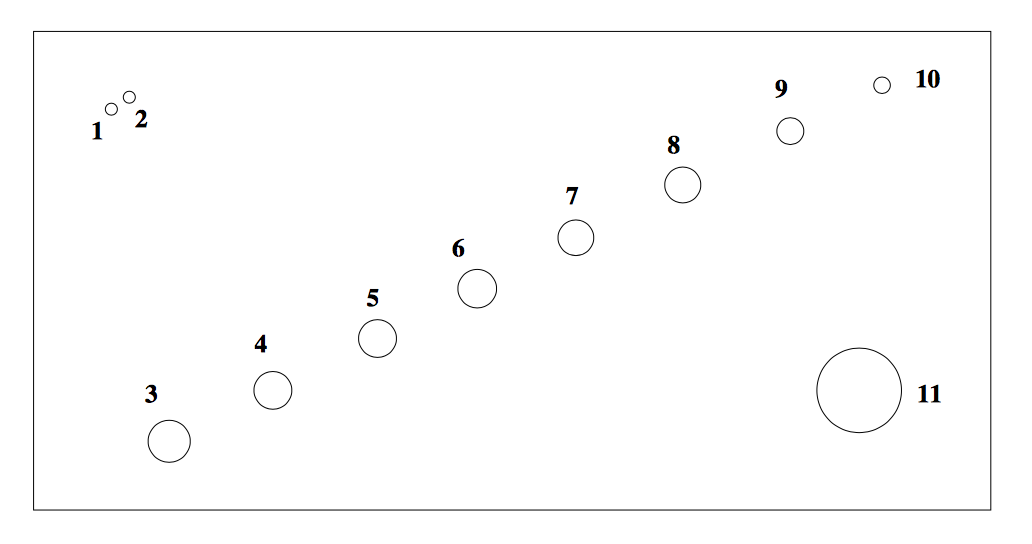
\includegraphics[scale=0.40]{fehlstellen.png}
  \caption{Darstellung der elf Fehlstellen.\cite{anleitung}}
  \label{fig:fehl}
\end{figure}
\newpage
Mithilfe des Impuls-Echo-Verfahrens wird im ersten Versuchsteil die Größe der einzelnen Fehlstellen
eines Acrylblocks untersucht.
Da die ersten beiden Fehlstellen sehr eng beieinander liegen, werden die Abmessungen
nochmal mit einer 2\,MHz Sonde aufgenommen.

Im zweiten Versuchsteil wird die Lage der Fehlstellen des Acrylblocks durch einen B-Scan bestimmt.
Dafür wird die 2\,MHz-Ultraschallsonde mit konstanter Geschwindkeit über den Acyrlblock bewegt.
Sowohl von unten als auch von oben wird der B-Scan durchgeführt.

Im letzten Versuchsteil wird der TM-Scan verwendet, um die Herzfrequenz und das Herzvolumen
eines Herzmodells zu bestimmen. Das Herzmodell wird zu einem Drittel mit Wasser gefüllt.
Die Sonde steht senkrecht mit der Wasseroberfläche in Kontakt. Die bewegliche Membran des
Modells ist mit einem Gummiball verbunden. Durch das Bewegen des Gummiballs kann das Herzpumpen
dargestellt werden. Mit dem TM-Scan wird dann die Volumenänderung sichtbar gemacht.
